\subsection{Long vowel headedness}
Whether long vowels are head-final or head-initial determines
if a language allows super-heavy Rhymes, i.e. whether Rhymes are
allowed to dominate up to three skeletal slots instead of only two.

If long vowels are head-initial, the second Nucleus has to be
licensed by a following nucleus, \TODO{}

\paragraph{In german:}
No alternation in vowel length $\to$ self-licensing $\to$ head-final

\TODO{Are super-heavy Rhymes allowed? (VVCC)}

p.~267:~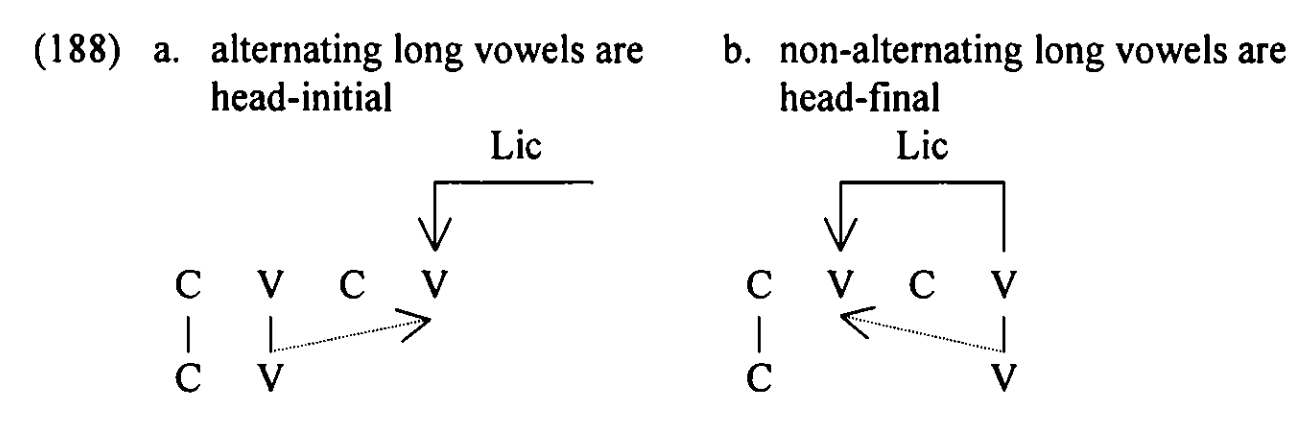
\includegraphics[width=.5\textwidth]{figures/long-vowel-headedness.png}


\subsection[Schwa]{Schwa\footnotemark}
  \footnotetext{
    In \cite{scheer2004}, \enquote{schwa} is defined phonologically
    as a vowel alternating with zero, with the added remark that for
    languages like German this \tr{fällt zusammen} with its phonetic
    reality: \textquote[{\cite[][p.~564]{scheer2004}}]{the alternating
    vowel is phonetically central and thus overtly deserves the name
    \enquote{schwa}}.
  }
Schwa does govern

Schwa does not license: \cite{scheer2004} analyzes the distribution
of \textipa{[N]} vs. \textipa{[Ng]} as an underlying \textipa{/\;Ng/}
where the \textipa{/g/} only surfaces if it is licensed.
In this analysis, three contexts are examined:

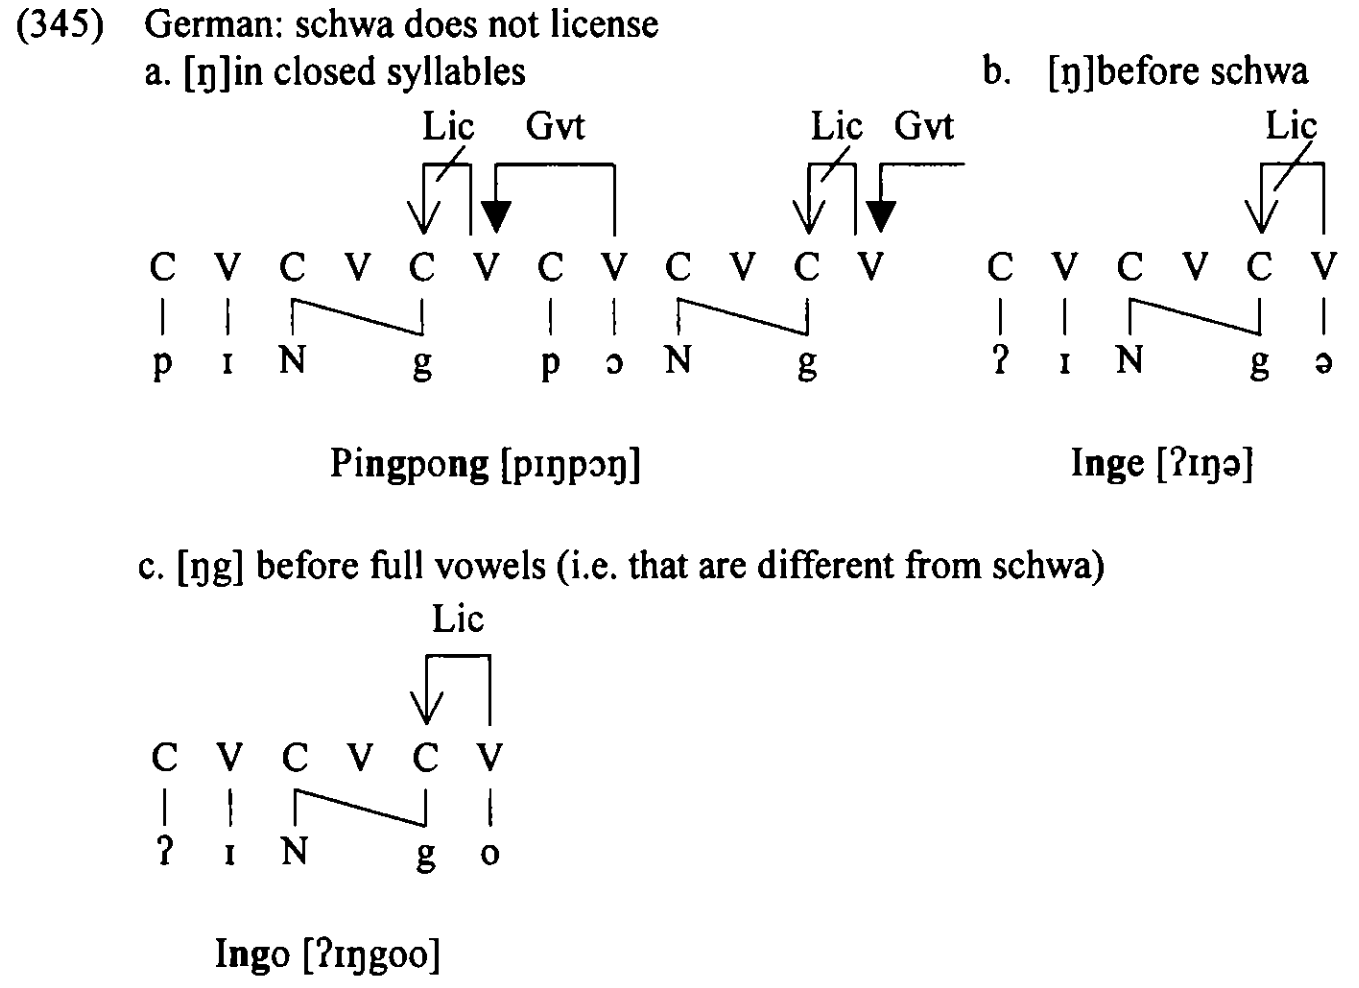
\includegraphics[width=.7\textwidth]{figures/ng-three-contexts.png}
(p.~580)

Since \textipa{/g/} doesn't surface before schwa it is concluded
that schwa doesn't license in German.


\subsection{FEN}
The lateral actorship of FEN can be determined by their effect

FEN do not license, FEN do govern


\subsection{Initial CV}


\subsection{Stress assignment}
\TODO{}